\documentclass[11pt,a4wide]{article}
\usepackage{verbatim}
\usepackage{listings}
\usepackage{graphicx}
\usepackage{a4wide}
\usepackage{color}
\usepackage[options]{SIunits}
\usepackage{amsmath}
\usepackage{amssymb}
\usepackage[dvips]{epsfig}
\usepackage[utf8]{inputenc}
\usepackage[OT1]{fontenc}
\usepackage{cite} % [2,3,4] --> [2--4]
\usepackage{shadow}
\usepackage{hyperref}

\setcounter{tocdepth}{2}
%
\lstset{language=c++}
\lstset{alsolanguage=[90]Fortran}
\lstset{basicstyle=\small}
\lstset{backgroundcolor=\color{white}}
\lstset{frame=single}
\lstset{stringstyle=\ttfamily}
\lstset{keywordstyle=\color{red}\bfseries}
\lstset{commentstyle=\itshape\color{blue}}
\lstset{showspaces=false}
\lstset{showstringspaces=false}
\lstset{showtabs=false}
\lstset{breaklines}

\begin{document}
\title{report on project $2$}
\author{Ekaterina Ilin and Isabelle Gauger\\GitHub: \url{https://github.com/CPekaterina/project-no2}
}
\maketitle
\tableofcontents
\newpage
\section{questions a)}
We look at the equation
\begin{equation}
\left|t\right| = \left|-\tau\pm\sqrt{1+\tau^2}\right|
\end{equation}
and consider the three cases $\tau=0$, $\tau>0$ and $\tau<0$.
For $\tau=0$ we get
\begin{equation}
\left|t\right| = \left|\pm1\right| = 1
\end{equation}
For $\tau>0$ the absolute value of $t$ is smaller for the solution with plus.  
\begin{equation}
\left|t\right| = \left|-\tau+\sqrt{1+\tau^2}\right|
\end{equation}
Now we look at $\tau\rightarrow\infty$:   
\begin{equation}  
\lim\limits_{\tau \rightarrow \infty}{\left|t\right|}=\lim\limits_{\tau \rightarrow \infty}{\left|-\tau+\sqrt{1+\tau^2}\right|}=0  
\end{equation}
For $\tau<0$ the absolute value of $t$ is smaller for the solution with minus.
\begin{equation}
\left|t\right| = \left|-\tau-\sqrt{1+\tau^2}\right|
\end{equation}
So now we look at $\tau\rightarrow-\infty$:
\begin{equation}
\lim\limits_{\tau \rightarrow -\infty}{\left|t\right|}=\lim\limits_{\tau \rightarrow -\infty}{\left|-\tau-\sqrt{1+\tau^2}\right|}=0  
\end{equation}
We have seen that for $\tau=0$ the absolute value of $t$ is one and if we increase or decrease $\tau$ it approachs zero.
\begin{equation}
\left|\tan{\theta}\right|\leq1 \text{for} \left|\theta\right|\leq\frac{\pi}{4}
\end{equation}
So if we choose $t$ to be the smaller of the roots $\left|\theta\right|\leq\frac{\pi}{4}$ what is minimizing the difference between the matrices A and B. This can be seen if we look at the given equation
\begin{equation}
||{\bf B}-{\bf A}||_F^2=4(1-c)\sum_{i=1,i\ne k,l}^n(a_{ik}^2+a_{il}^2) +\frac{2a_{kl}^2}{c^2}
\end{equation}
$(1-c)$ at the beginning of the equation becomes zero when $\cos{\theta}=1$ and than the total first part of the equation is zero. Also the second part of the equation reaches its minimum value for $\cos{\theta}=1$. For $\left|\theta\right|\leq\frac{\pi}{4}$ the value of $\cos{\theta}$ is between $1$ and $\approx 0.7$ so the difference between the matrices A and B we get is near the minimum. This means that the non-diagonal matrix elements of A are nearly zero, what is what we want to achieve.  
\section{Estimation of the execution time}
\begin{table}%
\centering
\caption{Number $N$ of similarity transformations performed in the Jacobi algorithm with respect to the dimensionality $n$ of the matrix. The ratio $N/n^2$ suggests a behaviour that can be written as $N(n)\approx a\cdot n^2$ with $a$ ranging in the order of $10^0$. More about the behaviour of $a$ in figure \ref{fig:a}.}
\begin{tabular}{lrr}\hline
$n$ & $N$ & $a=N/n^2$\\\hline
10 & 94 & 0.94\\
25 & 811 & 1.29\\
50 & 3542 & 1.42\\
100 & 14900 &1.49\\
500 & 386898 &1.55\\
1000 & $>10^6$ &-\\\hline
\end{tabular}
\label{tab:extime}
\end{table}
\begin{figure}[T]%
\centering
\includegraphics[scale=0.45]{b2.eps}%
\caption{The behaviour of the parameter $a$ in the $N(n)$ function that describes the number of similarity operations on the matrix can be approximated with an exponential function as shown in this figure.}%
\label{fig:a}%
\end{figure}
To estimate the number $N$ of similarity transformations performed we assume that the algorithm needs roughly $O(n^2)$ of the latter simply because each transformation sets a non-diagonal element to zero. The algorithm converges as shown above but in general we still may obtain up to $n-2$ new non-zero, non-diagonal matrix elements after every transformation. Therefore this assumption has to be verified numerically. Up to this point we have not yet considered the dependence of the convergence rate on the precision $\epsilon$ of the search for the maximal non-diagonal element.
\\
In the following discussion we set $\epsilon=10^{-12}$ and $\rho_ {max}=5$ and vary the dimensionality of the matrix in order to estimate the program's behaviour with respect to $n$.
\\
In table \ref{tab:extime} the number of similarity transformations is listed against the dimensionality $n$ of the matrix for some significant numbers. The range of $n$ is limited upwards due to the growth of the execution time, which goes with $n^3$. For $n=1000$ more than a million transformations are required and because each transformation takes $O(n)$ time the running time of the program falls outside of tolerance for greater $n$.
\\
From this table we conclude that the assumption made in the beginning is correct if we add a parameter $a$ to the function 
\begin{equation}
N(n)=a\cdot n^2
\label{eq:behofn}
\end{equation}
Let us now have a closer look at this parameter and assume a dependence on $n$, thus leading to
\begin{equation}
N(n)=a(n)\cdot n^2
\label{eq:a(n)}
\end{equation}
If we now plot $a$ against $n$ we can approximate its behaviour to a exponential decay function as shown in figure \ref{fig:a}. We note that in this model $a$ approaches the saturation limit for $n$ of the order of $10^2$ so that we can lean back and perform the algorithm for greater $n$ knowing that $a$ should not change significantly. But, however, more computational power is needed to verify this theory.

\section{dependency on the choice of $\rho_{max}$}
To find out how the accuracy of the computed eigenvalues depends on the choice of $\rho_{max}$ we computed the lowest three eigenvalues for $n=50$ steps and different values of $\rho_{max}$. For $\rho_{max}$ between $4$ and $20$ the difference between the computed eigenvalues and the correct solutions is smaller than $1.0$. If we start with $\rho_{max}=4$ and make it smaller and smaller the error increases until the computed eigenvalues are totally different from the correct solution. The same happens when we start with $\rho_{max}=20$ and make it bigger and bigger. To find the $\rho_{max}$ for which the error of the computed eigenvalues becomes minimal we focused on the area $4<\rho_{max}<20$. We computed the difference between the three lowest eigenvalues and the correct solutions for $\rho_{max}=4,5,6,..,10,15,20$, which is shown in table \ref{tab:n=50 dif. rho_max}.

\begin{table}%
\centering
\caption{Difference between the lowest three computed eigenvalues and the correct solutions for $n=50$ and different $\rho_{max}$}
\begin{tabular}{lrrrr}\hline
$\rho_{max}$ & error ev1 & error ev2 & error ev3 & error total\\\hline
4	& 0.00197	& 0.00665	& 0.0529 & 0.06152\\
5	& 0.00313	& 0.01566	& 0.0381 & 0.05689\\
6	& 0.00451	& 0.02257	& 0.0552 & 0.08228\\
7	& 0.00614	& 0.03077	& 0.0752 & 0.11211\\
8	& 0.00802	& 0.04024	& 0.0985 & 0.14676\\
9	& 0.01016	& 0.05101	& 0.125	 & 0.18617\\
10 & 0.01256	& 0.06308	& 0.1547 & 0.23034\\
15 & 0.02842	& 0.14367	& 0.3549 & 0.52699\\
20 & 0.05095	& 0.26008	& 0.6501 & 0.96113\\\hline
\end{tabular}
\label{tab:n=50 dif. rho_max}
\end{table}

\begin{table}%
\centering
\caption{Difference between the lowest three computed eigenvalues and the correct solutions for $n=100$ and different $\rho_{max}$}
\begin{tabular}{lrrrr}\hline
$\rho_{max}$ & error ev1 & error ev2 & error ev3 & error total\\\hline
4 & 0.00047 & 0.00088 & 0.0724 & 0.07375\\
5 & 0.00078 & 0.00391 & 0.0093 & 0.01399\\
6 & 0.00113 & 0.00563 & 0.0137 & 0.02046\\
7 & 0.00153 & 0.00766 & 0.0187 & 0.02789\\
8 & 0.002   & 0.01001 & 0.0245 & 0.03651\\
9 & 0.00253 & 0.01269 & 0.031  & 0.04622\\
10 & 0.00313 & 0.01566 & 0.0383 & 0.05709\\ 
15 & 0.00705 & 0.03534 & 0.0865 & 0.12889\\
20 & 0.02842 & 0.14367 & 0.3549 & 0.52699\\\hline
\end{tabular}
\label{tab:n=100 dif. rho_max}
\end{table}

\begin{table}%
\centering
\caption{Difference between the lowest three computed eigenvalues and the correct solutions for $n=200$ and different $\rho_{max}$}
\begin{tabular}{lrrrr}\hline
$\rho_{max}$ & error ev1 & error ev2 & error ev3 & error total\\\hline
4 &	0.0001	& 0.00276	& 0.0772	& 0.08006\\
5	& 0.0002	& 0.00097	& 0.0022	& 0.00337\\
6	& 0.00028	& 0.00141	& 0.0034	& 0.00509\\
7	& 0.00038	& 0.00191	& 0.0047	& 0.00699\\
8	& 0.0005	& 0.0025	& 0.0061	& 0.0091\\
9	& 0.00063	& 0.00317	& 0.0077	& 0.0115\\
10	& 0.00078	& 0.00391	& 0.0095	& 0.01419\\
15	& 0.00176	& 0.0088	& 0.0215	& 0.03206\\
20	& 0.00313	& 0.01566	& 0.0383	& 0.05709\\\hline
\end{tabular}
\label{tab:n=200 dif. rho_max}
\end{table}

The total error is minimal for $\rho_{max}=5$. To see if this is also the case for other numbers of steps we did the same for $n= 100,200$. As table \ref{tab:n=100 dif. rho_max} and \ref{tab:n=200 dif. rho_max} show the total error is also minimal for $\rho_{max}=5$ when we choose $n=100$ or $n=200$. For $\rho_{max}=5$ $279$ steps are needed to get the three lowest eigenvalues with four leading digits. For other values of $\rho_{max}$ more steps are needed. 

\section{comparison with function tqli}
To compare the results of our jacobi algorithm with the function tqli in the file lib.cpp we computed the lowest three eigenvalues for $\rho_{max}=5$ and $n=50,100,200,400$. The results are shown in table \ref{tab:rho_max=5 dif. n jacobi} and \ref{tab:rho_max=5 dif. n tqli}.

\begin{table}%
\centering
\caption{lowest three eigenvalues for $\rho_{max}=5$ and different numbers of steps with jacobi algorithm}
\begin{tabular}{lrrr}\hline
N & ev1 & ev2 & ev3\\\hline
50 &	2.99687	& 6.98434	& 10.9619\\ 
100	& 2.99922	& 6.99609	& 10.9907\\ 
200	& 2.9998	& 6.99903	& 10.9978\\ 
400	& 2.99995	& 6.99976	& 10.9996\\\hline
\end{tabular}
\label{tab:rho_max=5 dif. n jacobi}
\end{table}

\begin{table}%
\centering
\caption{lowest three eigenvalues for $\rho_{max}=5$ and different numbers of steps with tqli}
\begin{tabular}{lrrrr}\hline
N & ev1 & ev2 & ev3\\\hline
50 & 2.99687	& 6.98434	& 10.9619\\ 
100	& 2.99923	& 6.9961	& 10.9907\\ 
200	& 2.9998	& 6.99904	& 10.9978\\ 
400	& 2.99994	& 6.99978	& 10.9999\\\hline 
\end{tabular}
\label{tab:rho_max=5 dif. n tqli}
\end{table}      
The eigenvalues computed with jacobi and tqli are nearly equal. The biggest difference between them is $0.0003$ for the third eigenvalue with $n=400$. The execution time of the two algorithms for $\rho_{max}=5$ and different numbers of steps is shown in figure \ref{fig:execution time}. For small numbers of steps both algorithms need nearly the same time but already for $n=200$ tqli is twice as fast as the jacobi algorithm. For $n=400$ it is more than three times as fast as jacobi. 
\begin{figure}[T]%
\centering
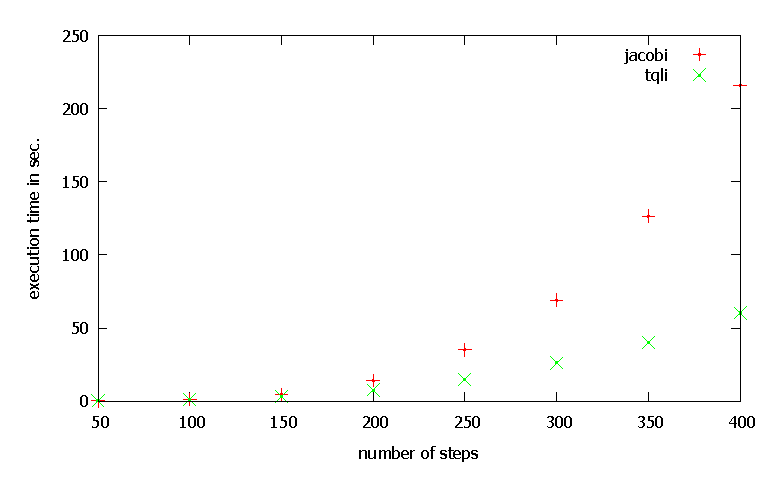
\includegraphics[scale=0.45]{execution_time.eps}%
\caption{execution time of jacobi and tqli for $\rho_{max}=5$ and different numbers of steps}%
\label{fig:execution time}%
\end{figure}
\end{document}
   
